\subsection{Machine Learning \--- Reformulation}

\subsubsection{Aim}

\begin{frame}
\frametitle{Reformulation: a translation module}

\begin{figure}
 \begin{tikzpicture}
  \node (0) at (10,10) {$\triple$};
  \onslide<1>{\node (1) at (10,8.5) {\alert{president}};}
  \node (2) at (12,8.5) {?};
  \node (3) at (8,8.5) {$\triple$};
  \node (4) at (8,7) {United States};
  \onslide<1>{\node (5) at (5,7) {\alert{birth date}};}
  \node (6) at (10,7) {?};

  \onslide<1>{\draw[->, >=latex] (0) edge node[sloped, anchor=center, above] {\scriptsize{pred.}} (1);}
  \draw[->, >=latex] (0) edge node[sloped, anchor=center, above] {\scriptsize{obj.}} (2);
  \draw[->, >=latex] (0) edge node[sloped, anchor=center, above] {\scriptsize{subj.}} (3);
  \onslide<1>{\draw[->, >=latex] (3) edge node[sloped, anchor=center, above] {\scriptsize{subj.}} (5);}
  \draw[->, >=latex] (3) edge node[sloped, anchor=center, above] {\scriptsize{obj.}} (6);
  \draw[->, >=latex] (3) edge node[sloped, anchor=center, above] {\scriptsize{pred.}} (4);

  \onslide<2>{\node (7) at (10,8.5) {\alert{birth date}};}
  \onslide<2>{\node (8) at (5,7) {\alert{president}};}
  \onslide<2>{\draw[->, >=latex] (0) edge node[sloped, anchor=center, above] {\scriptsize{pred.}} (7);}
  \onslide<2>{\draw[->, >=latex] (3) edge node[sloped, anchor=center, above] {\scriptsize{subj.}} (8);}

  \onslide<1>{\draw[<->, >= latex] [draw=mLightBrown] [bend right=50, above] (1) edge (5);}
  
 \end{tikzpicture}
\end{figure}

%Changing the form, not the content.
\end{frame}

\subsubsection{Operation}
\begin{frame}
\frametitle{Operation}
\alert{Projection:} trees $\mapsto$ vector space.

The dictionary associates a vector triple to a vector.
\end{frame}

\begin{frame}
\frametitle{Projection}
\begin{center}
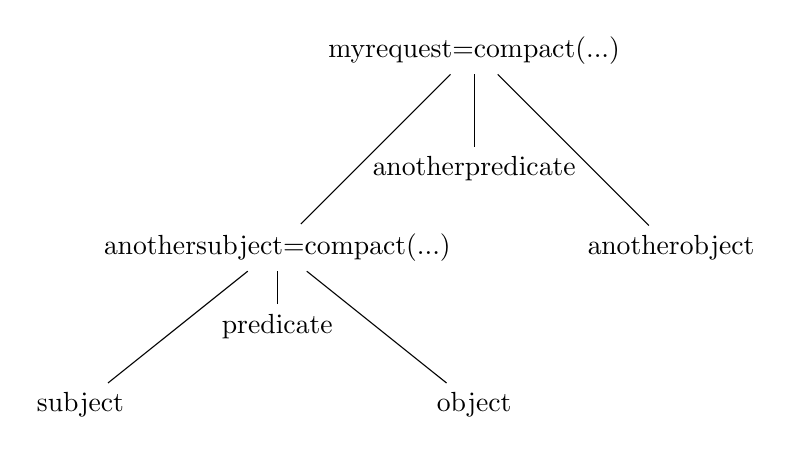
\begin{tikzpicture}[x=2.5cm]
\node (s) at (1,0) {subject};
\node (p) at (3,0) {object};
\node (r) at (2,1) {predicate};


\node (a) at (2,2) {anothersubject=compact(...)};
\node (b) at (4,2) {anotherobject};
\node (l) at (3,3) {anotherpredicate};
\node (h) at (3,4.5) {myrequest=compact(...)};

\draw (s)--(a)--(p);
\draw (r)--(a);
\draw (a)--(h)--(b);
\draw (l)--(h);
\end{tikzpicture}
\end{center}
\end{frame}

\subsubsection{Build the request}

\begin{frame}
\frametitle{From vector to tree}

\begin{center}
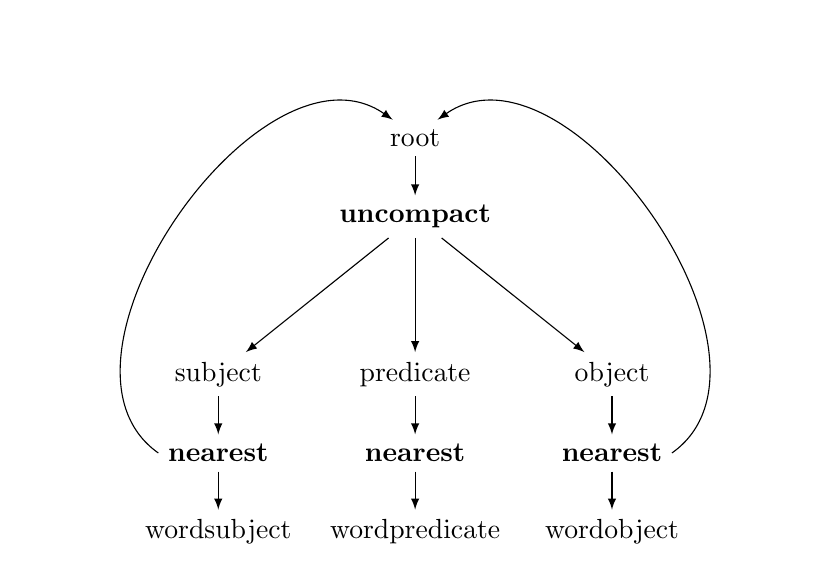
\begin{tikzpicture}[x=2.5cm]
\node (s) at (1,0) {subject};
\node (p) at (3,0) {object};
\node (r) at (2,0) {predicate};
\node (sf) at (1,-1) {\textbf{nearest}};
\node (pf) at (3,-1) {\textbf{nearest}};
\node (rf) at (2,-1) {\textbf{nearest}};
\node (sw) at (1,-2) {wordsubject};
\node (pw) at (3,-2) {wordobject};
\node (rw) at (2,-2) {wordpredicate};
\node[rectangle] (b) at (2,2) {\textbf{uncompact}};
\node (v) at (2,3) {root};
%\node (b) at (4,2) {b};
%\node (l) at (3,3) {l};
%\node (h) at (3,4) {h=compact(a,l,b)};

\draw[->, >=latex] (b)--(s);
\draw[->, >=latex] (b)--(p);
\draw[->, >=latex] (b)--(r);
\draw[->, >=latex] (v)--(b); % WTF?
\draw[->, >=latex] (r)--(rf);
\draw[->, >=latex] (p)--(pf);
\draw[->, >=latex] (s)--(sf);
\draw[->, >=latex] (rf)--(rw);
\draw[->, >=latex] (pf)--(pw);
\draw[->, >=latex] (sf)--(sw);

\draw [->, >=latex] (pf.east)        to [bend right=90] (v);
\draw [->, >=latex] (sf.west)        to [bend left=90] (v);
\end{tikzpicture}
\end{center}
\end{frame}

\subsubsection{Learn}

\begin{frame}
\frametitle{Training}
\alert{Semantic distance.}

Use relation graph ``instance of'' from Wikidata.
\end{frame} 
